%%%%%%%%%%%%%%%%%%%%%%%%%%%%%%%%%%%%%%%%%%%%%%%%%%%%%%%%%%%%%%%%%%%
%                                                                 %
%                            CHAPTER THREE                        %
%                                                                 %
%%%%%%%%%%%%%%%%%%%%%%%%%%%%%%%%%%%%%%%%%%%%%%%%%%%%%%%%%%%%%%%%%%%

\chapter{CONCEPTUAL MODEL}

The conceptual model used within this thesis is built around the expression of three core versioning operations: addition, invalidation, and modification.  These three activities can be represented by interacting with three types of concepts: versions, attributes, and changes.  Versions represent the data entities being compared.  These could be two different editions of a book or versions of software.  It is important to understand that a version is an abstraction as it can be represented by multiple physical files.  In the sections that follow, operations will only consider the interaction between two versions and will be explained later in the chapter.  Versions then contain attributes representing a quantity being modified.  Specifically for tabular data, attributes would correspond to an identifier that refers to particular rows or columns within the data.  Attributes of the two versions are then connected by a change.  This link functions as a very general concept which can be subclassed into more informative types such as unit changes, improving the expressiveness of the model beyond PROV's revisionOf concept.

\section{ADDITION}

When a change adds a new attribute to a version, it only needs to refer to version two and its corresponding attribute.  The reasoning should be fairly obvious as the attribute never existed in version one, and therefore, there is nothing to refer to and no need to form a relationship between the change and version one.  However, by linking the addition change to version one, we address a difficulty with comparing provenance graphs.  When two data objects have identical structures, it is difficult to determine what time the objects were added to the dataset and which version they belong to.  As a result, determining the compatability of the two objects becomes difficult.  The change contributions to the dataset evolution appears naturally using this construction. The resulting model can be seen in Figure~\ref{AdditionFig}.

\begin{figure}
	\centering
	\vspace{0.0in} % normally the command here would be \includegraphics
%	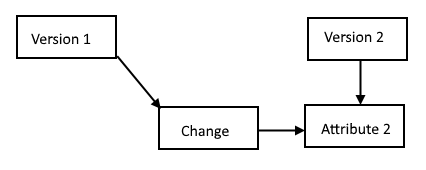
\includegraphics{figures/Addition.png}
	\begin{tikzpicture}[every node/.style={draw, rectangle}]
		\begin{scope}[node distance=20mm and 20mm]
			\node (c) [scale=1.25] at (1,0) {Change A};
			\node (1) [above left=of c, scale=1.25] {Version 1};
			\node (2) [above right=of c, scale=1.25] {Version 2};
			\node (a) [below =of 2, scale=1.25] {Attribute 2};
			
			\draw [line width=2pt,->] (1) -- (c);
			\draw [line width=2pt,->] (c) -- (a);
			\draw [line width=2pt, ->] (2) -- (a);
		\end{scope}
	\end{tikzpicture}
	\caption{Model of the relationships between Versions 1 and 2 when adding an Attribute 2 to Version 2 as a result of Change A}
	\label{AdditionFig}  % the \label command comes AFTER the caption
\end{figure}



\section{INVALIDATION}

The Invalidation operation corresponds to the delete concept found in other applications.  The choice of invalidation over delete results from the policy that data is never deleted.

\begin{figure}
	\centering
	\vspace{0.0in} % normally the command here would be \includegraphics
	%	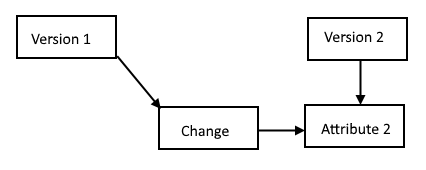
\includegraphics{figures/Addition.png}
	\begin{tikzpicture}[every node/.style={draw, rectangle}]
	\begin{scope}[node distance=20mm and 20mm]
	\node (c) [scale=1.25] at (1,0) {Change I};
	\node (1) [above left=of c, scale=1.25] {Version 1};
	\node (2) [above right=of c, scale=1.25] {Version 2};
	\node (a) [below =of 1, scale=1.25] {Attribute 1};
	
	\draw [line width=2pt,->] (a) -- (c);
	\draw [line width=2pt,->] (c) -- (2);
	\draw [line width=2pt, ->] (1) -- (a);
	\end{scope}
	\end{tikzpicture}
	\caption{Model of the relationships between Versions 1 and 2 when invalidating Attribute 1 from Version 1 as a result of Change I}
	\label{Invalidationfig}  % the \label command comes AFTER the caption
\end{figure}


\section{MODIFICATION}

\section{MULTIPLE LINKED VERSIONS}
